%%% -*-LaTeX-*-

\chapter{Solution Counting}

Today, SweetPea offloads the entire sampling process to an external tool. While an attractive option from an implementation standpoint, this strategy does not scale to the degree needed by SweetPea. As demonstrated in Chapters 1 and 3, the solution spaces from which SweetPea is trying to sample are beyond the capacity of any existing tools. One of the shortcomings of this approach is that external tools cannot exploit domain knowledge of the problem to guide their decisions.

One may view experimental designs in SweetPea as combinatorics problems, each with a countable set of solutions. If a formula for counting the solutions to an experimental design could be derived, then it may also be possible to discover a bijection between solutions to the design and the natural numbers. If a corresponding natural number could uniquely identify every possible solution, then we could guarantee uniformity by randomly sampling natural numbers from the uniform distribution. As a first foray into solution counting, this chapter presents such a formula for tier one, two, and three designs. This exploration will also defer treatment of the set of external design constraints.


\section{Principles of Counting}

Before describing a formula for counting solutions to experimental designs, it will be useful to review a few counting principles for future reference, beginning with counting permutations of a set. As explained by Brualdi \cite{brualdi_introductory_2010}, the standard formula for computing the number of permutations of $r$ items taken from an $n$-element set is:

\[
P(n,r) = \frac{n!}{(n-r)!}
\]

When $n =  r$, this becomes simply $n!$.

% Similary, the number of combinations of $r$ items from an $n$-element set is:

% \[
% {n \choose r} = \frac{n!}{r!(n-r)!}
% \]

When constructing a set $S$ by combining individual elements from mulitple other sets, $P_1, P_2, \cdot\cdot\cdot P_n$, the size of $S$ is the product of the sizes of sets $P_1, P_2, \cdot\cdot\cdot P_n$:

\[
|S| = \prod_{i=1}^n |P_i|
\]

This is known as the \textit{Multiplication Principle} \cite{brualdi_introductory_2010}. Both of these principles will be used to calculate the number of solutions to a SweetPea design.


\section{Partition of an Experimental Design}

An experimental design is composed of three elements: a set of factors, a subset of the factors that form the crossing, and a set of constraints. The set of crossed factors fundamentally shapes the generated trial sequences. The number of combinations of level values taken from each crossed factor governs the length of a trial sequence. For example, consider a design in which there are two crossed factors, each with three levels. By the multiplication principle, there are $3 * 3 = 9$ unique combinations of level values from each factor in the crossing; hence, trial sequences in this design will be nine trials long. The sequence length is a critical factor in the solution count, as are other factors that are not in the crossing.

To formalize the relationship between each factor and the total solution count, we define a partition for the set of factors in the design. Let $D$ be the set of all factors in the design. Let $C$ be the set of factors that form the crossing, and $\overline{C}$ be the set of factors not included in the crossing. Therefore $C \subseteq D$ and $\overline{C} \subset D$. We can further divide $C$ and $\overline{C}$ by basic and derived factors. Let $C_B$ be the set of basic factors in $C$, and $C_D$ be the set of derived factors in $C$. $\overline{C}_B$ and $\overline{C}_D$ are defined as the basic factors not in the crossing and the complex factors not in the crossing respectively.

Lastly, we further divide $\overline{C}_B$ into two more sets. Although the set of crossed factors does not include basic factors in $\overline{C}$, this does not imply that they are fully independent. Factors in $\overline{C}_B$ may contribute to the selected levels for factors in $C_D$. We will refer to these factors in $\overline{C}_B$ as \textit{source} factors, as they are at least a partial source of data controlling factors in $C_D$. We will group such factors in $\overline{C}_{B_S}$, while $\overline{C}_{B_I}$ represents the truly independent basic factors in $\overline{C}$.

We could also define $C_{B_S}$ and $C_{B_I}$, however, there is no benefit to doing so. Because the crossing is the highest source of authority, the relationship between factors in $C_B$ and dependent derived factors is inverted. Each combination of levels in the crossed set governs the values for $C_B$, which will then, in turn, govern dependent derived factors.

The partition of $D$ with which we are concerned is therefore: $\{C_B, C_D, \overline{C}_{B_S}, \overline{C}_{B_I}, \overline{C}_D\}$. A visual hierarchy of this partition is shown in Figure \ref{fig:partition}.

% \begin{figure}[t]
% \centering
% \centerline{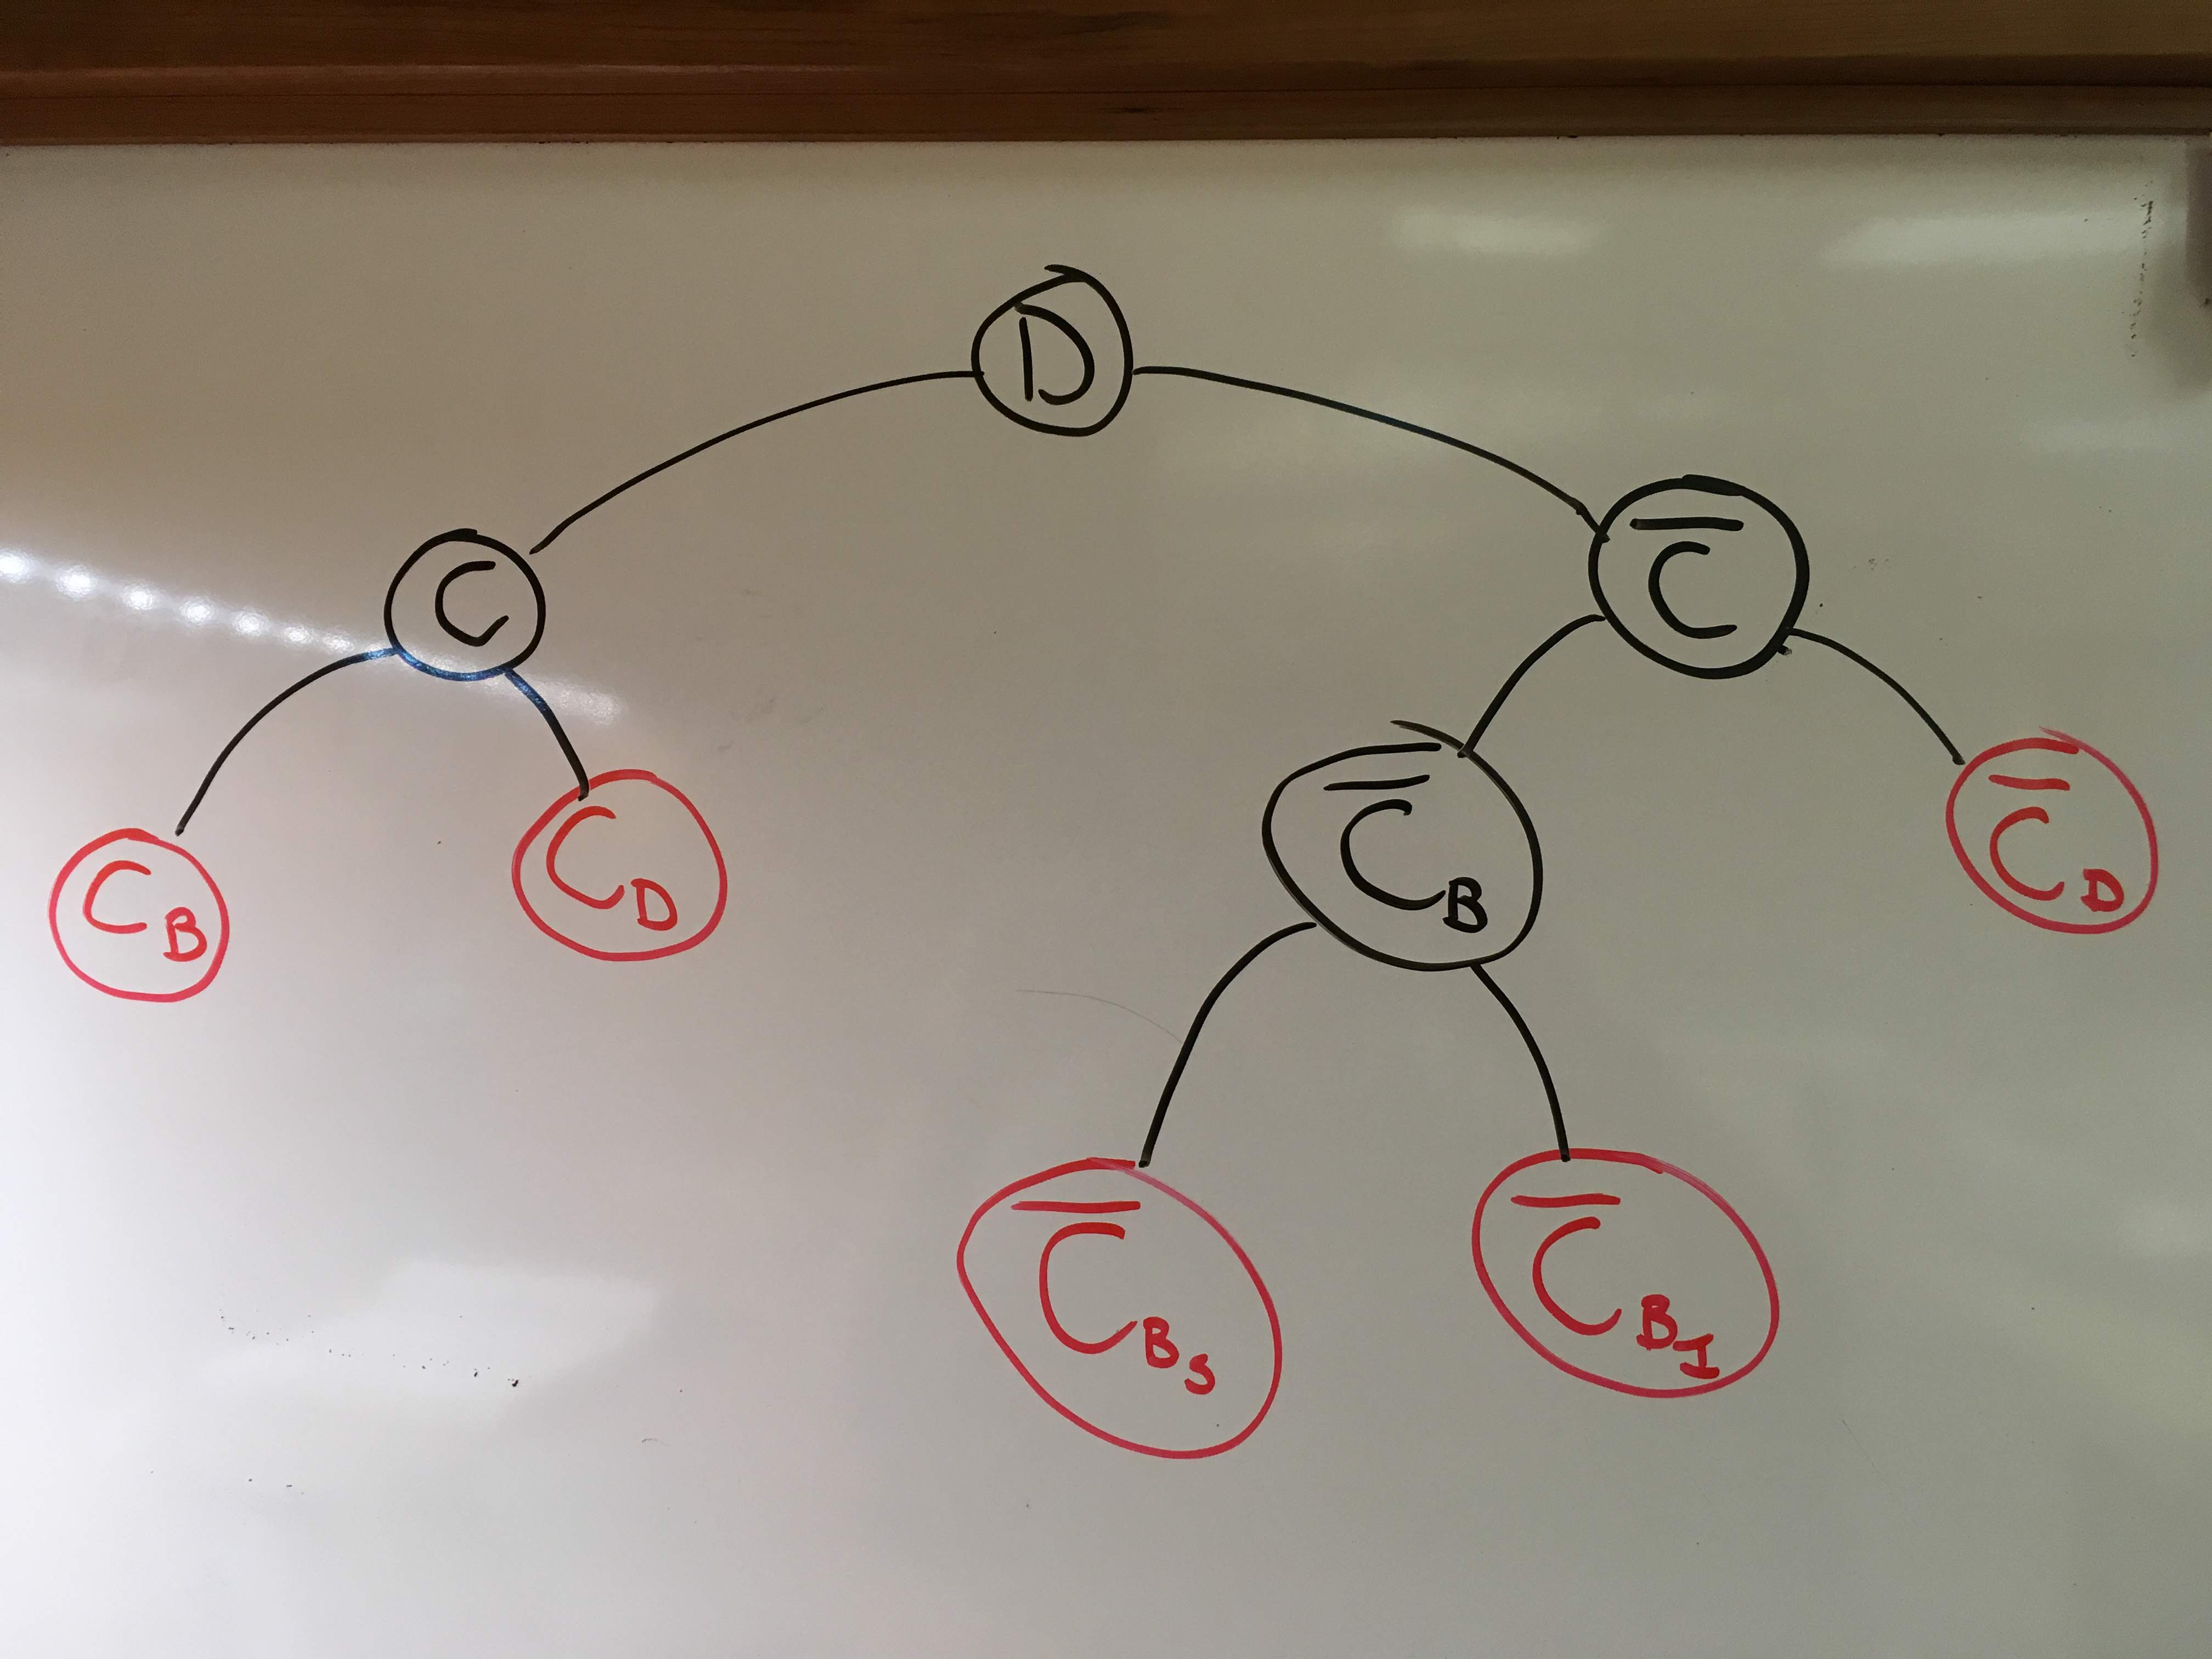
\includegraphics[origin=c,width=12cm]{../figures/partition.jpg}}
% \caption{Partition of an Experimental Design}
% \label{fig:partition}
% \end{figure}

\begin{figure}[b]
\centering
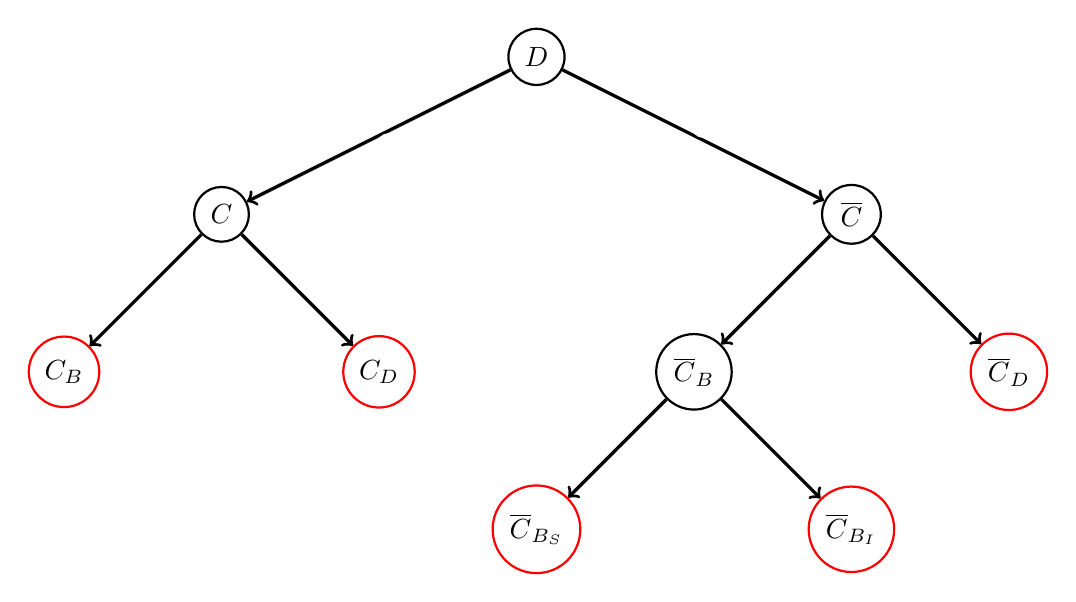
\begin{tikzpicture}[auto]
\begin{scope}[every node/.style={circle,thick,draw}]
    \node (D) at (8,8) {$D$};

    \node (C) at (4,6) {$C$};
    \node (CBar) at (12,6) {$\overline{C}$};

    \node[draw=red] (CB) at (2,4) {$C_B$};
    \node[draw=red] (CD) at (6,4) {$C_D$};
    \node (CBarB) at (10,4) {$\overline{C}_B$};
    \node[draw=red] (CBarD) at (14,4) {$\overline{C}_D$};

    \node[draw=red] (CBarBS) at (8,2) {$\overline{C}_{B_S}$};
    \node[draw=red] (CBarBI) at (12,2) {$\overline{C}_{B_I}$};
\end{scope}

\begin{scope}[every node/.style={fill=white,circle},
              every edge/.style={draw=black,very thick}]
    \path [->] (D) edge node {} (C);
    \path [->] (D) edge node {} (CBar);

    \path [->] (C) edge node {} (CB);
    \path [->] (C) edge node {} (CD);

    \path [->] (CBar) edge node {} (CBarB);
    \path [->] (CBar) edge node {} (CBarD);

    \path [->] (CBarB) edge node {} (CBarBS);
    \path [->] (CBarB) edge node {} (CBarBI);
\end{scope}
\end{tikzpicture}
\caption{Partition of an Experimental Design}
\label{fig:partition}
\end{figure}


Lastly, we establish notation for referrings to individual level combinations in $C$. Let $X$ be a set of sequences $t_1, t_2, \cdot\cdot\cdot t_n$, representing the combinations of levels for all factors in $C$. Each sequence $t$ contains items $i_1, i_2, \cdot\cdot\cdot i_j$, where item $i_j$ is one of the levels from the $j_{th}$ factor in $C$. Each sequence $t$ must be unique, and there is an sequence for every possible combination of levels from factors in $C$.

Recall the earlier design example with factors to represent the color and text of a printed word. Both the color and text factors had three levels: \texttt{red}, \texttt{green}, and \texttt{blue}. For this crossing, $X$ can be visualized in Table \ref{tab:sequences}.

\begin{table}[htb]
  \centering
  \caption{Expressing Level Combinations as Sequences}
\begin{tabular}{|c|cc|}
\hline
\textbf{}      & \textbf{$i_1$} & \textbf{$i_2$} \\ \hline
\textbf{$t_1$} & red            & red            \\
\textbf{$t_2$} & red            & green          \\
\textbf{$t_3$} & red            & blue           \\
\textbf{$t_4$} & green          & red            \\
\textbf{$t_5$} & green          & green          \\
\textbf{$t_6$} & green          & blue           \\
\textbf{$t_7$} & blue           & red            \\
\textbf{$t_8$} & blue           & green          \\
\textbf{$t_9$} & blue           & blue           \\   \hline
\end{tabular}
\label{tab:sequences}
\end{table}

By the multiplication principle, there will be $n = C_1 \cdot C_2 \cdot\cdot\cdot C_{|C|}$ such sequences, and there are $P(n, n) = n!$ permutations of this set. We will also use $l$ to refer to the trial sequence length, which is equivalent to $|X|$.


\section{Formula}

With the partition established, we can develop the formula for counting the number of solutions, $s$, for a given experimental design. We will first derive the formula for a tier 1 design, and then add additional terms for tier 2 and tier 3 designs.

\subsection{Tier 1}

For tier 1 designs, the sequences in $X$ fully represent all possible level combinations in the design. $C_B \neq \emptyset$, while every other set in the partition is empty. The only variation between trial sequences is the ordering of pairs in $X$. Therefore, every permutation of $X$ represents a unique trial sequence, which means there are $s = l!$ solutions to a tier 1 design.

\subsection{Tier 2}

Tier 2 designs allow basic factors that are not in $C$, and are thus less constrained. In otherwords, starting with tier 2, $\overline{C}_{B_I} \neq \emptyset$. For a factor $f$, let $|f|$ denote the number of levels that $f$ has. For each $f \in \overline{C}_{B_I}$, $f$ is fully independent; therefore, any of the $|f|$ levels may be selected for each trial. In a sequence of $l$ trials, applying the multiplication principle reveals that there are $|f|^l$ possible sequences of levels of $f$. If $|\overline{C}_{B_I}| > 1$, then the multiplication principle is applied repeatedly to determine the total number of combinations for all factors in $\overline{C}_{B_I}$. Applying the multiplication principle a final time produces the final formula for tier 2:

\[
s = l! \cdot \prod_{i=1}^{|\overline{C}_{B_I}|} |f_i|^l
\]

\subsection{Tier 3}

Tier 3 designs allow the addition of derived factors. It is now possible that all sets in the partition are non-empty. $C_D$, $\overline{C}_{B_S}$, and $\overline{C}_D$ are the only sets in the partition remaining to account for. The presence of factors in $C_D$ does not alter the formula, as level selection for factors in $C_D$ is still controlled by $X$ (the crossing), regardless of their relationship to other factors. $\overline{C}_D$ also requires no special treatment as the level selection for uncrossed derived factors depends entirely on the levels selected for basic factors. (Regardless of whether the basic factors are in $C_B$, $\overline{C}_{B_S}$, or $\overline{C}_{B_I}$.) Only $\overline{C}_{B_S}$ remains, containing the uncrossed basic factors that feed crossed derived factors.

Derived factors allow the user to provide an arbitrary predicate for each level in the factor. SweetPea applies these predicates to every combination of levels that could be given as arguments, effectively constructing a truth table, to determine which level to select for each combination of arguments. We define $X_S$ to be the set of sequences representing the crossing of factors in $\overline{C}_{B_S}$, also referred to as the \textit{source crossing}. The next task is to determine, for every element in $X$, which elements of $X_S$ are compatible using the user-defined predicates. Checking compatibility is necessary as some combinations in $X$ may preclude certain combinations in $X_S$.

For every sequence $t \in X$, there is some number of elements in $t$ corresponding to derived factor levels, labeled $d_1, d_2, \cdot\cdot\cdot d_{|C_D|}$ comprising the set $V_t$. Each $d \in V$ is associated with a predicate,\footnote{These predicates, also called derivation functions, are expected to be deterministic. If they are non-deterministic, then inconsistent solutions may be produced as the predicates may be applied more than once to the same arguments. SweetPea could minimize this concern by ensuring that each predicate is only applied once to each argument combination and then caching the results.} $pred(d)$. For every $t \in X$, every $b \in X_S$ is consulted to see if the predicates for all $d \in V_t$ are satisfied.\footnote{If $X$ is very large, then testing all combinations could become intractable. However in practice, $X$ is relatively small, typically $|X| < 500$. Additionally, SweetPea's current implementation relies on $X$ being small enough for this to work, as it follows a similar process when generating the SAT encoding for derived factors.} If any of them is not satisfied, then $b$ is not a compatible choice for $t$ and must be discarded from consideration for $t$. Once this process is complete, a list of subsets of $X_S$ remains, in which the $n^{th}$ subset indicates which elements of $X_S$ are compatible with the $n^{th}$ crossing in $X$.

More formally, let $S$ be a list of items $J_1, J_2, \cdot\cdot\cdot J_{|X|}$. The following statements are true:

\begin{enumerate}
\item $\forall J \in S \mid J \subseteq X_S$
\item $\forall t \in X,  \forall d \in V_t \mid pred(d) \implies \top$
\end{enumerate}

Once we have generated $S$, we can apply the multiplication principle once more to complete the formula for tier 1, 2, and 3 designs:

\[
s = l! \cdot \prod_{i=1}^{|\overline{C}_{B_I}|} |f_i|^l \cdot \prod_{k=1}^{|S|} |J_k|
\]

The total number of solutions $s$ for a given experimental design is the product of the number of permutations of the crossing, the number of combinations of each independent factor, and the number of acceptable combinations of all source factors.

It is possible for the user to specify a crossing that is not satisfiable. Referring back to the Stroop example, the user may include all three factors, \texttt{color}, \texttt{text}, and \texttt{congruent}, in the crossing. This is unsatisfiable because some level combinations violate the rules of the derived factor. For example, \texttt{color=red}, \texttt{text=blue}, and \texttt{congruent=yes} is invalid because \texttt{red} and \texttt{blue} are not congruent according to the predicates for \texttt{congruent}. If such a crossing is specified, the formula for $s$ will correctly identify the number of potential solutions as zero.

\section{Example}

Consider a design composed of the same factors as the Stroop example:

\begin{verbatim}
color = Factor("color", ["red", "green", "blue"])
text  = Factor("text",  ["red", "green", "blue"])

congruent = Factor("congruent?", [
    DerivedLevel("yes", WithinTrial(operator.eq, [color, text])),
    DerivedLevel("no",  WithinTrial(operator.ne, [color, text]))
])
\end{verbatim}

However, rather than crossing \texttt{color} and \texttt{text}, we will demonstrate an example in which \texttt{color} and \texttt{congruent?} are crossed. For this design, the partition of $D$ becomes:

\begin{gather*}
    C_B = \{\texttt{color}\} \quad C_D = \{\texttt{congruent?}\}  \quad  \overline{C}_{B_S} = \{\texttt{text}\} \\
    \overline{C}_{B_I} = \emptyset \qquad\qquad \overline{C}_D = \emptyset
\end{gather*}

The crossing, or $X$, is the cartesian product of levels of \texttt{color} and \texttt{congruent?}. SweetPea generates this product exhaustively.

\begin{align*}
X = \{(red, yes), (red, no), (green, yes), (green, no), (blue, yes), (blue, no)\}
\end{align*}

The size of the crossing determines the sequence length, therefore $l = |X| = 6$. As a result, the first term, $l!$, becomes $6! = 720$.

In this design, there are no basic independent factors outside the crossing: $\overline{C}_{B_I} = \emptyset$. Therefore there is no value for the second term.

For the third and final term, we need to first determine $X_S$, the cartesian product of levels of factors in $\overline{C}_{B_S}$. For this design, the only factor in $\overline{C}_{B_S}$ is \texttt{text}. As a result, $X_S$ is simply the levels in \texttt{text}:

\[
X_S = \{red, green, blue\}
\]

At this point, each element of the product of $X$ and $X_S$ must be checked for validity under the derived factor definitions in the design to determine the subsets of $X_S$ that are valid for each element in $X$. In terms of this example, which level selections in $X_S$ do \textit{not} violate the definition of \texttt{congruent?} when paired with each level selection combination in $X$? These subsets comprise $S$ as defined in Section 4.3.3. Table \ref{tab:example_s} gives a visual representation of this process.

\begin{table}[b]
  \centering
  \caption{Computing $S$ for Solution Counting}
\begin{tabular}{r|c|c|c|c}
\cline{2-4}
\multicolumn{1}{c|}{}              & \multicolumn{3}{c|}{$X_S$}                 & \multicolumn{1}{l}{}                     \\ \hline
\multicolumn{1}{|c|}{$X$}          & red          & green        & blue         & \multicolumn{1}{c|}{$J$}                 \\ \hline
\multicolumn{1}{|r|}{(red, yes)}   & $\checkmark$ &              &              & \multicolumn{1}{c|}{$\{(red\}$}         \\ \hline
\multicolumn{1}{|r|}{(red, no)}    &              & $\checkmark$ & $\checkmark$ & \multicolumn{1}{c|}{$\{(green, blue)\}$} \\ \hline
\multicolumn{1}{|r|}{(green, yes)} &              & $\checkmark$ &              & \multicolumn{1}{c|}{$\{(green\}$}       \\ \hline
\multicolumn{1}{|r|}{(green, no)}  & $\checkmark$ &              & $\checkmark$ & \multicolumn{1}{c|}{$\{(red, blue)\}$}   \\ \hline
\multicolumn{1}{|r|}{(blue, yes)}  &              &              & $\checkmark$ & \multicolumn{1}{c|}{$\{(blue\}$}        \\ \hline
\multicolumn{1}{|r|}{(blue, no)}   & $\checkmark$ & $\checkmark$ &              & \multicolumn{1}{c|}{$\{(red, green)\}$}  \\ \hline
\end{tabular}
\label{tab:example_s}%
\end{table}

$S$ is therefore:

\[
S = \{(red), (green, blue), (green), (red, blue), (blue), (red, green)\}
\]

With $S$ defined, we may now compute the third term of the formula:
\[
    \prod_{k=1}^{|S|} |J_k| = 1 \cdot 2 \cdot 1 \cdot 2 \cdot 1 \cdot 2 = 8
\]

This yields the final solution count of $s = 720 \cdot 8 = 5,760$. One may confirm this solution by generating the corresponding SAT encoding for this design and applying a model counter to the generated CNF.

\section{Conclusion}

In this chapter, we derived a formula for counting the number of solutions to SweetPea designs in tiers 1, 2, or 3. However, this formula does not account for the third component of a design: constraints. Including constraints in the formula is beyond the scope of this thesis, as it would involve complexity similar to counting solutions for tier 4 and five designs. The formula, therefore, produces an exact solution count for designs lacking constraints and produces an upper-bound for designs with constraints. Next, we will apply the counting formula to construct uniformly-distributed trial sequences without relying on a SAT sampler.

% TODO: Correctness proof? Mention that we tested counts with SAT model counters?
